\section{Implementation}
% Exact PVSS scheme choice and parameters (concrete curve, primes, etc.),
% state the complexity.

We implement all on-chain components of the non-incentivized scheme in Solidity and off-chain components in Typescript and Rust.
We use SCRAPE~\cite{pvss_scrape} as the underlying PVSS scheme by adapting the implementation given by Gurkan et al.~\cite{aggregatable_dkg}.
Since SCRAPE relies on Type 3 pairings, our PVSS ciphertext is instantiated using the curve BN254~\cite{bn254}, as at the time of writing only it is the only curve with Type 3 pairings available as precompiles on Ethereum.
Similar to the scheme presented by Schoenmakers~\cite{pvss_schoenmakers}, SCRAPE's dealer shares the secret $s$ but the committee recovers $h^s$, where $h$ is the generator of $\mathbb{G}_2$ in BN254.
Therefore, our implementation of the scheme requires the dealer to produce $\hat{c}$ by encrypting $m$ with the truncated SHA256 hash of a $h^s$ rather than use $s$ directly.

Though BN254 is not a SNARK friendly curve, we have optimized the proving time of the zkSNARK circuit from Algorithm \ref{alg:snark_circuit} by leveraging the fact that SCRAPE's instantiation of \textsf{PVSS.verifyDist} allows us to be convinced that $\textsf{PVSS.genDist}(s, [pk_i]) = c$ just by checking $F_0 = g^s$ (where $g$ is the generator of $\mathbb{G}_1$).
Since \textsf{PVSS.verifyDist} already checks consistency of $F_0$ with the rest of the ciphertext, we only need to check whether $\log F_0 = s$.
This involves only one BN254 exponentiation inside of Algorithm \ref{alg:snark_circuit} and makes the circuit size constant, allowing proving time to be constant.
To optimize the proving time of the zkSNARK further, we compress the problem instance by first hashing $(c, \mathcal{R}, x)$ before passing it into $H$, and instantiate $H$ using Poseidon~\cite{poseidon}, a SNARK friendly hash function.
The primary bottleneck of performance is \textsf{PVSS.verifyDist}, which occurs on chain and has optimal $O(n)$ complexity using SCRAPE.

% Experimental methodology (Ethereum mainnet, Solidity, give GitHub link / open source license).

% Gas cost VS committee size
We use a Hardhat node to measure the on-chain gas cost paid for by the dealer in $\textsf{WE.Encrypt}_\mathcal{R}$, relative to $n$ and $t$.
As can be seen in Figure~\ref{fig:gas_cost}, the maximum committee size that does not consume more gas than the block gas limit is 56. 
The code for the implementation can be found at \url{https://github.com/galletas1712/cassiopeia}.
\begin{figure}\label{fig:gas_cost}
\caption{Gas cost of \textsf{encrypt} vs committee size}
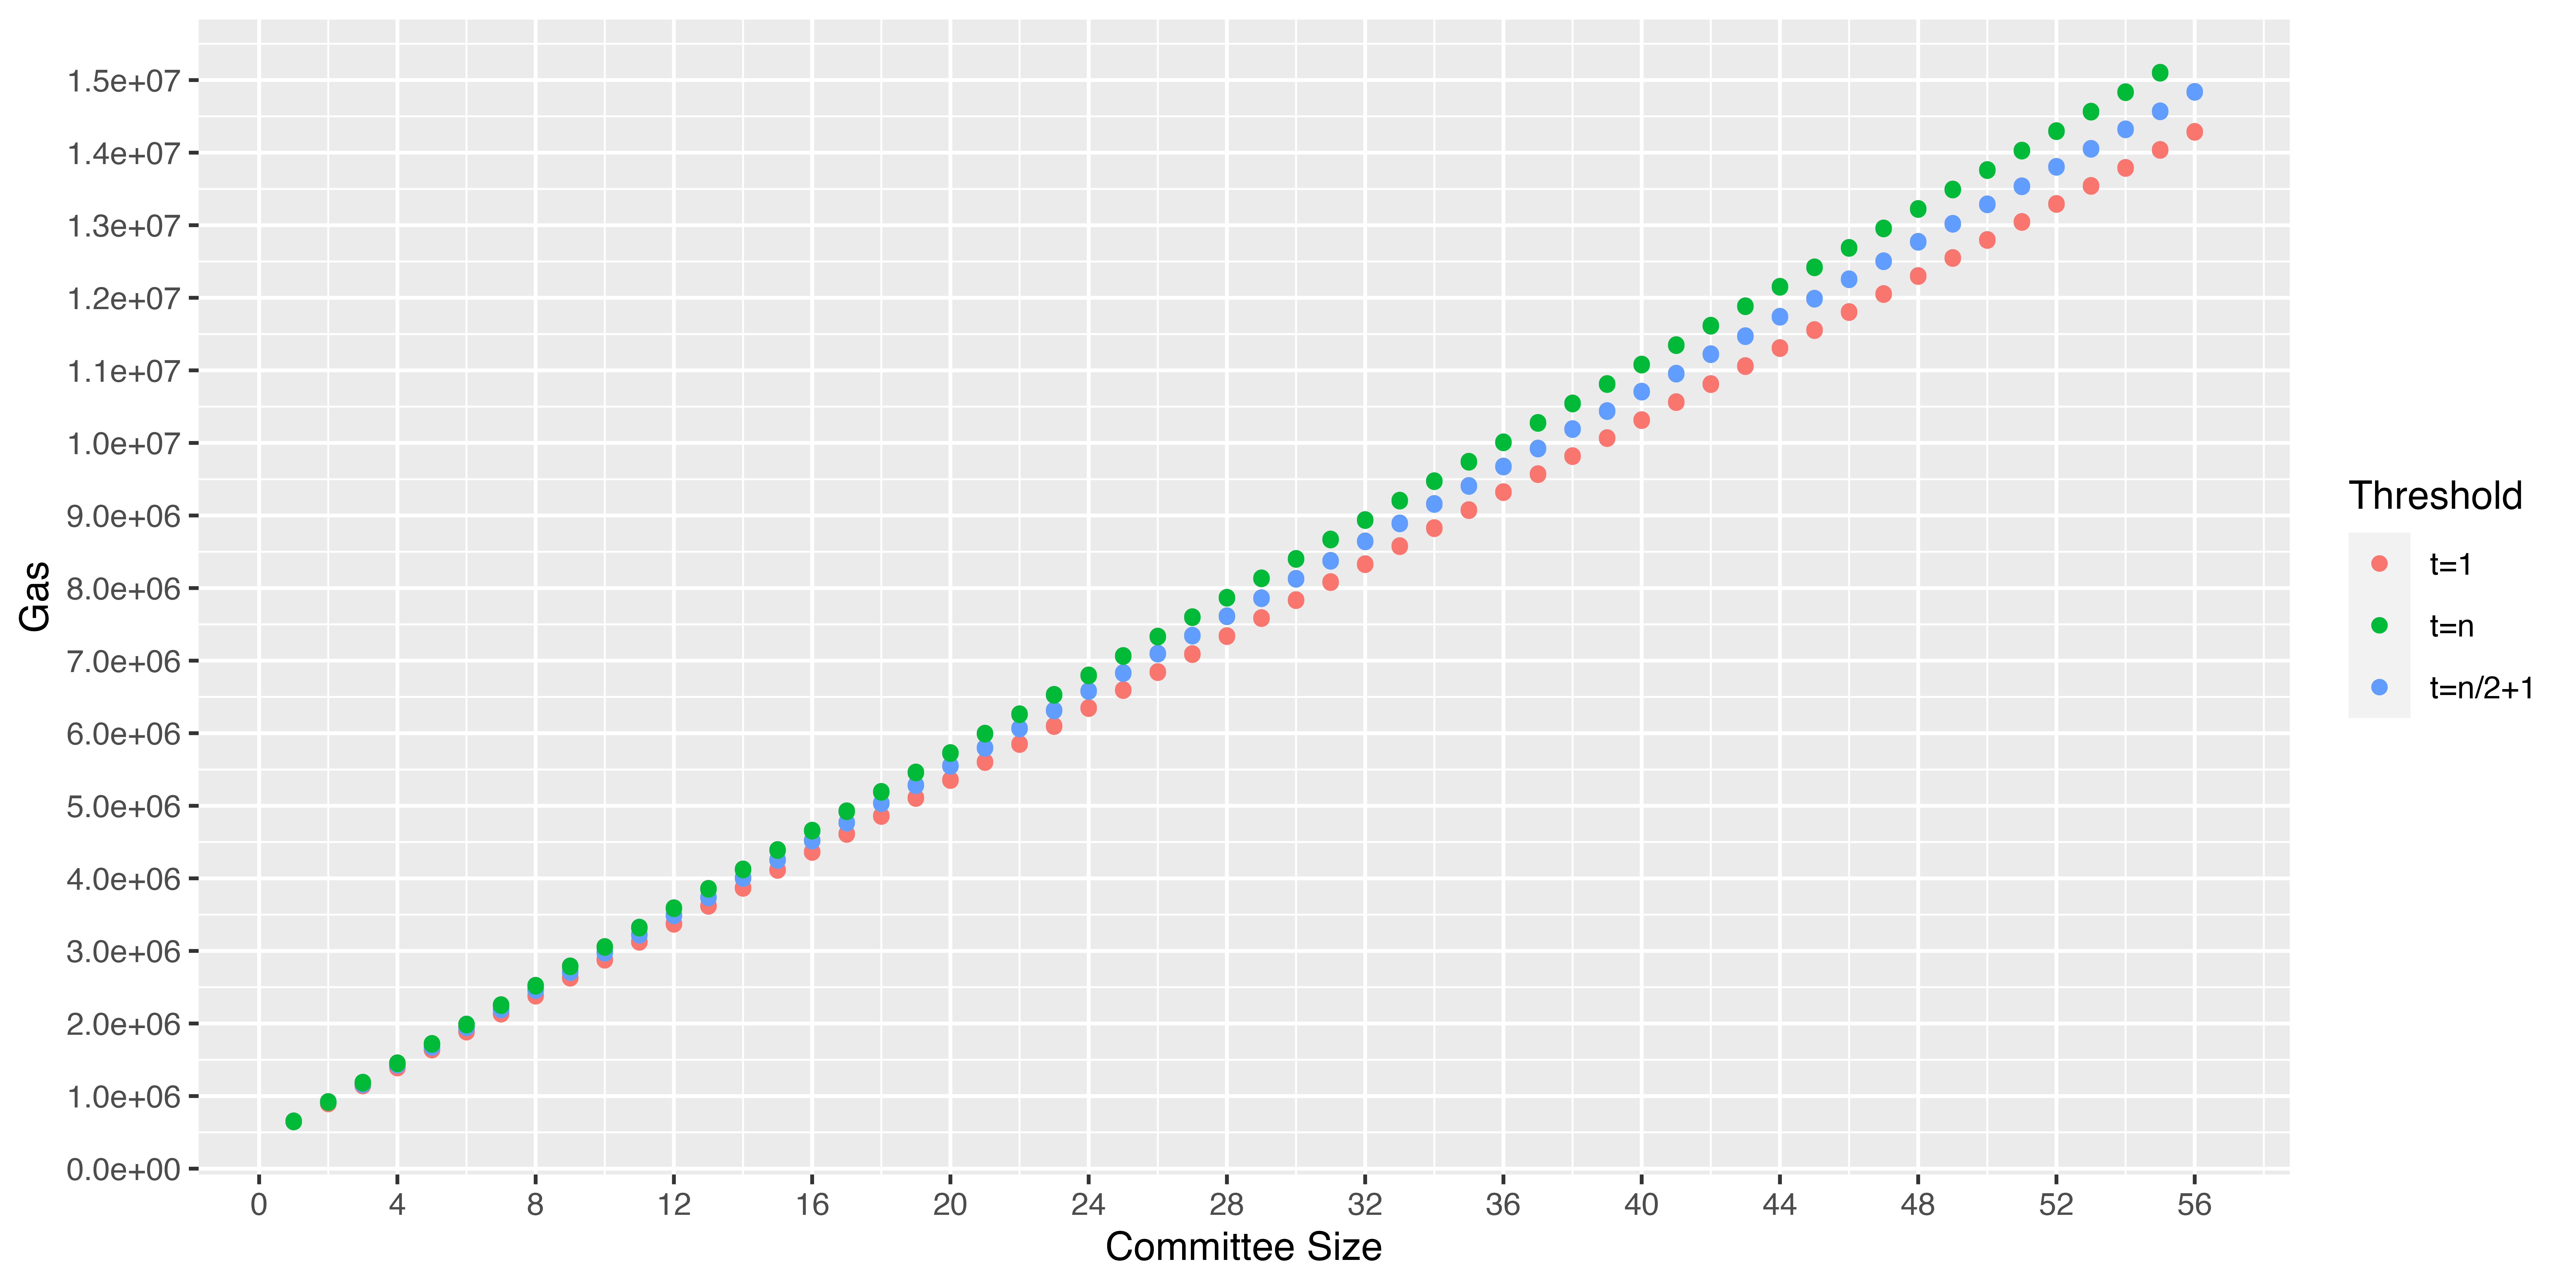
\includegraphics[width=1.15\textwidth]{gas_cost}
\end{figure}

% TODO: Offchain computation time VS committee size

